\documentclass{article}
\usepackage[margin=2cm]{geometry}
\usepackage{graphicx}
\usepackage{hyperref}
\usepackage{caption}
\usepackage{float}
\usepackage{setspace}
\usepackage{cite}

\begin{document}

\title{Design Document for 4D Tetris Project}
\author{Your Name}
\date{\today}
\maketitle

\tableofcontents
\newpage

\section{Overview of the Project}
% Approximate Word Count: 200 words

In this project I will try to develop a 4 dimensional variant of Tetris. The game will try to capture the essence of the original Tetris gameplay as well as the endless replayability while enhancing it with innovative new features. To find a balance in between the increased complexity provided by moving into higher dimensional spaces and the actual playability end enjoyability of the game, I will be limiting the 4 dimensional aspect to the Tetris pieces only. The player will see a 3 dimensional playing field that pieces fall into. Once they start rotating the 3 dimensional pieces they will notice that they are actually 3 dimensional slices of 4 dimensional collections of hypercubes. This will essentially just increase the number of possible rotations of the pieces and remove the rotational symmetry that is present in classic Tetris.
The goal is to create a fun fut complex game that lends itself to endless replayability as well as scientific exploration, just as Tetris did.

\section{Project Template Used}
% Approximate Word Count: 50 words
CM3030 Games Development Project Idea Title 1: Arcade Game

\section{Domain and Users of the Project}
% Approximate Word Count: 300 words
\subsection{Gamers}
I will try to capture a wide audience for this game. Tetris is played by young and old, people from different educational backgrounds and different cultures.
As described by Csikszentmihalyi \cite{flow} this can be done by creating a state of flow. To induce this state several things must be true.
\begin{enumerate}
    \item A challenging activity that requires skill
    \item Clear goals and feedback
    \item The player must be able to concentrate on the task at hand
    \item Direct and immediate feedback
    \item A sense of control
    \item A loss of self-consciousness
    \item An altered sense of time
\end{enumerate}
When looking at this list, it is clear that Tetris succeeded in all of them. The biggest chalange for this project will be to make it easy enough so users of all backgrounds can achieve 'flow'. As Chen \cite{flow_2} stated this can be achieved, by unlocking additional choices (pieces) when the player has obtaines some suffiency. Some users will struggle with the basic concept of higher dimensions, and the game is required to ease them into a basic understanding of how the rotations work. Others will have no issues getting into the game but will require additional challanges to be sucked into the game and keep engaged. The game needs to create a sense of reward in users playing it for 5 minutes during a short break as well as users that are willing to invest several hours to achieve higher scores. Due to the nature of the game it is expected that it will have a somewhat larger appeal on users with advanced education, so these will be the primary focus group during evauation, however, previous projects into the same realm have shown that focussing solely on this group will not be enough to create a successful game. Targeted testing will be carried out, and I will try to include at least 25\% of the testers from a group with a lower educational background.
\subsection{Research}
A secondary target user group will be the academic community. Tetris has been widely used as a research subject. Our variant will rely heavily on mental rotation and spatial reasoning, both have been an important part of psychological reasearch \cite{COOPER197520} \cite{CORBALLIS1997100} \cite{Kornhaber_2020} \cite{Lau_zhu}. This could be a very interested target audience if the game itself implements features that aid researchers in experiment design. Voice of customer will be conducted in advance of development to gain insights into what specific features would be suitable to engange the scientific community.
This might be as simple as exporting pieces spawned + keystrokes into a csv file.
% Explain the domain (e.g., educational gaming) and describe the target users.

\section{Justification of Design Choices}
% Approximate Word Count: 350 words
Several choices had to be made during envisioning.
\subsection{4D}
While it was very enticing to try to implement a fully 4 dimensional game and or move tha play field into 4D as well. Preliminary user research as well as an extensive review of previous work has shown that this would increase the comlpexity to a level where the likelyhood of overall commercial success for such a project would decrease dramatically due to a decease in target users and the total obtainable market. I will therefore limit the playingfield to 3 dimensions and the pieces to 3 dimensional slices of 4 dimensional objects.
\subsection{Gameplay}
Due to limitations when it comes to user input the interactions within the 4th dimension will be limited. To be precise ther will be no way to move the w plane and change the slice we are prohecting into 3d space. The w plane will always be in the middle. This does however leave and opening for later expansion/enhancment of the gameplay.
\subsection{User Interface}
I feel that it is necessary to create a very informative user interface due to the complexity of the game and the fact that the arrow keys will have different functionalities depending on which action key is pressed. This shall be achieved through graphical overlays that will inform the player of the type of rotation/movement that will be performed in the current state.
\subsection{Scoring}
For the prototype multiline tetrises will be disabled. The primary goal of the MVP is to establish fun and engaing gameplay.
\subsection{Art Style}
The art style will be very important for the game. While people with higher educational background will likely be enticed by the mere concept of a 4 dimensional game, other user groups will need appealing and contemporary visuals to be kept enganged.


% Explain how your design decisions meet user needs and fulfill domain requirements.

\section{Overall Structure of the Project}
% Approximate Word Count: 350 words
The game will be made out of several components that will interact with each other. The main components are:
\subsection{GameManager}
This will take care of the overall game state. It will keep track of the current score, the current level, the current piece, the next piece, the playing field and the current state of the game. 
\subsection{HyperCube}
The basic building block of the game. This will be a 4 dimensional extension of a cube. It will be used to procedurally generate the mesh userd for rendering the pieces as well as basic rotation logic. Collision detection will be done in 3 dimensional space.
\subsection{Piece}
This will be a 4 dimensional collection of hypercubes. the main rotational logice be implemented here. The current plan is to decimpose the piece once it is resting on the playing field. In addition the rendering will switch from wireframe to solid. With individual cubes rendered in a color accorading to the row they are on.
\subsection{Block}
This will be the collection of all resting cubes and will be used for the detection of completed planes.
\subsection{Level}
This is the playing field. Will generate the mesh, keep track of the block and give options for later enlargement of the playing field (not in MVP).
\subsection{User Interface}
Will be a column on the right containing scores, level etc. as well as an overlay that will help the user understand the rotations.
\subsection{InputManager}
Will switch between different state depending on the action key pressed chaning the functionality of the arrow keys and relaying the information to the pieces.
\subsection{AudioManager}
Will take care of the audio. Will be very basic in the MVP.

% Describe the architecture, including main components and their interactions.

% Include diagrams (not counted in word limit).
\begin{figure}[H]
    \centering
    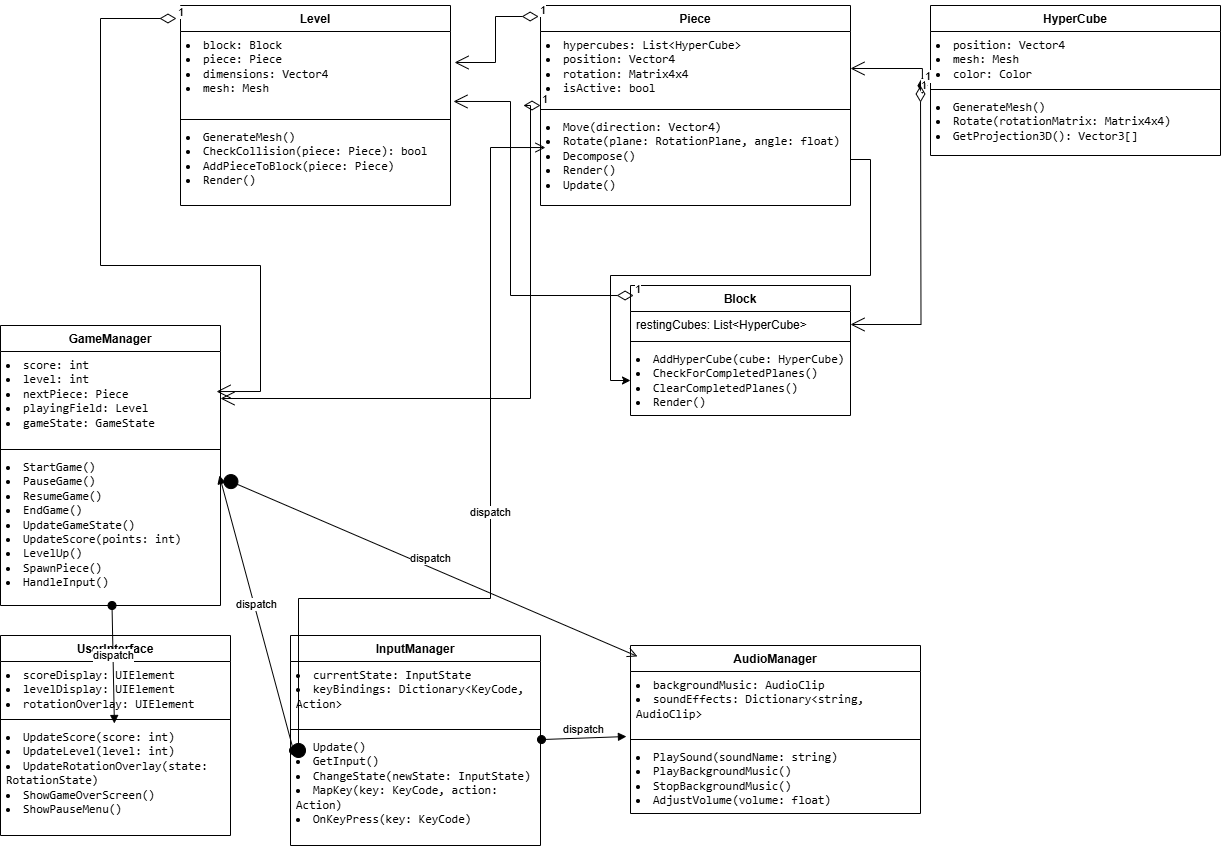
\includegraphics[width=\textwidth]{classes.png}
    \caption{Overall Architecture of the 4D Tetris Project}
    \label{fig:architecture}
\end{figure}

\section{Important Technologies and Methods}
% Approximate Word Count: 300 words

% Identify key technologies, algorithms, and justify their use.

\section{Plan of Work}
% Approximate Word Count: 250 words

% Outline major tasks and timeline.

% Include Gantt chart (not counted in word limit).
\begin{figure}[H]
    \centering
    %\includegraphics[width=\textwidth]{gantt_chart.png}
    \caption{Project Timeline Gantt Chart}
    \label{fig:gantt}
\end{figure}

\section{Testing and Evaluation Plan}
% Approximate Word Count: 250 words

% Describe how you will test and evaluate the project.

\newpage

\appendix

\section{References}
% Include any references used (not counted in word count).
%\begin{thebibliography}{9}
%\bibitem{ref1} Author Name, \textit{Book Title}, Publisher, Year.
%\bibitem{ref2} Article Author, ``Article Title,'' \textit{Journal Name}, vol., pp., Year.
%\end{thebibliography}
\bibliographystyle{acm}
\bibliography{references}

\section{Additional Figures and Diagrams}
% Include any additional images or diagrams here.

\end{document}
